\chapter{Linear Functions}

Now that we have a good understanding of what a function is, it's time to begin exploring one of the most common types of functions: the linear function.


\begin{defn}[Linear Function]\label{Line}
	A linear function is a function that increases at a constant rate. The \hyperref[Solution Set]{solution set} of a linear function is an infinite number of points. 
\end{defn}


\section{Slope-Intercept Form}

When the equation of a linear function takes the form
\begin{equation}
f(x) = mx + b
\end{equation}

\noindent
we say it is in slope-intercept form.  When we're looking at equivalent equations, this form is one of the most useful for plotting the line, because when we choose a value for $x$, the right side of the equation turns into an expression that we can simplify to find $f(x)$.  This form of an equation also contains useful information that we can use to make plotting lines faster.  The $m$ is the slope.  The $b$ is the vertical-intercept. 

Notice that $y$ is not being included in this formula. There is a reason for that. We want to think about these lines as representations of functions. Therefore, throughout this chapter, the vertical axis will sometimes be referred to as the $f(x)$ axis and the coordinates will sometimes be referred to as an $x$ coordinate and a $f(x)$ coordinate (in the form $(x, f(x))$. This works the same as you might be used to, but with this notation, we have more flexibility with what variables we use. Whether we use the variable $y$ or the function notation $f(x)$, we are talking about the output of a function. 

	
\begin{defn}[Slope]
	The slope of a line is a number representing how steep the line is. It is calculated by finding the rate of change of the function. The higher the value of the slope, the steeper the line is. A negative slope indicates that, as the x-value increases, the line slants downward.
\end{defn}

The rate of change is a central idea to understanding functions. For functions in general, we find the average rate of change by looking at the change in output and dividing that by the change in input.
\[
\text{Average Rate of Change}=\frac{\triangle \text{output}}{\triangle \text{input}}
\]

\noindent
But when we are dealing with lines, the rate of change is always constant. So instead of finding the average rate of change, we can find the exact rate of change. 

\begin{example}[Finding the Slope from a Graph]\label{Slope on a graph}
	\begin{center}
	\begin{tikzpicture}
	\begin{axis}		%Uncommenting the following line and putting it on this line with no space results in an error.
	%[axis background/.style={fill=white}, width=12cm, ymax=10, ymin=-10, xmax=10, xmin=-10, axis lines=middle, grid=major, myaxis, xticklabel style= {font=\tiny, yshift=0.5ex}, yticklabel style={font=\tiny, xshift=0.5ex},xtick={-10,...,10}, ytick={-10,...,10}]
	\addplot+[smooth] coordinates {(-9,-8) (9,5)};
	\end{axis}
\end{tikzpicture}
	\end{center}
	
Here we have a linear function, graphed on the domain of $[-9,9]$. If we are asked to find the slope(or rate of change) of this function, we have all the information we need on the graph. If the rate of change is $\frac{\triangle\text{output}}{\triangle\text{input}}$, then how would we find our slope?
\end{example}


Unfortunately, we don't always have a beautiful picture to look at to find the slope.  Sometimes, we only have some points that we can use.  However, if we're told that these points are on a linear function, we can use the same kind of reasoning to find the slope.  Since each point has an $x$ and a $f(x)$ value, we'll use those in what we call the slope formula.

It's valuable to remember that order is important.  If Angelica has 3 cookies today, and 2 cookies tomorrow, the change in cookies is 1, but when we're talking about lines, we need to know if the number went up one or down one.  We find differences by subtracting, so we need to make sure we choose the right order for subtracting one value from the other.  Here, we would want to subtract the value of today from the value of tomorrow, to make sure we have a negative number, to show that the number went down by one.

The same applies to points.  When we want to find the change in $x$, we want to be careful to choose which point is first and which one is second.  It won't matter which is which as long as you keep the $x$ and $f(x)$ values together.

\begin{equation}
m = \frac{f(x_2) - f(x_1)}{x_2 - x_1}
\end{equation}

\begin{example}

If we have two points, (2,3) and (5,6), we want to choose one point to be first.  Let's have (2,3) be first.  Each point has an $x$ and a $f(x)$ value, so the first point's $x$-value is 2.  We call this value $x_1$ in the formula.  The second points $x$-value is 5, and we call it $x_2$.  This pattern gives us everything we need to plug into the formula.  However, we need to be careful to use to the same order when we use the $f(x)$-values.  $f(x_1)$ is 3, and $f(x_2)$ is 6.  When we plug these in, $$m = \frac{6 - 3}{5 - 2}$$

We can then simplify this to $\frac{3}{3}$, which simplifies further to 1.  This tells us that the line that these points come from has a slope of 1.
\end{example}



\section{Point-Slope Form}

As we've learned previously, for any equation, there are countless equivalent equations.  In addition to having a slope-intercept form, equations also have a point-slope form.  If equations in slope-intercept form use the valuable information of slope and intercept, what kinds of information can we get from a line in point-slope form?

The point-slope form of a line looks like the following.

\begin{equation}
y - k = m(x-h)
\end{equation}

In this form, m is still the slope, but we have two new values, h and k.  These are the x and y values of a point on the line, (h,k).  This form of a line is sometimes useful to find, but more often it is used as a formula to plug values into.  As its name suggests, if you have the slope of a line and a point on it, you can find the equation of the line.

\begin{example}
If a line has slope 1 and passes through the point (2,3), what is the equation of the line in slope-intercept form?

We take the information we are given and understand that, with the point and the slope, we use the point-slope form of the line, and we can plug those values straight in.

The point (2,3) is our point (h,k) from the form of the line.  So we take the equation $y - k = m(x - h)$ and plug them in, to get $y - 3 = m(x - 2)$.  We also take the slope, 1, and plug it in for m to get $y - 3 = 1(x - 2)$.  Now the we have no variables other than x and y, we can solve for y. to get the slope-intercept form.

$y - 3 = x - 2$

$y = x + 1$

\end{example}

With all of the information we have so far, we can find the y-intercept, slope, equation, and any points we need from a graph of a line.  We can also find the y-intercept, slope, equation, and graph from only two points on the line.  The most valuable skill for learning this is the concept of equivalent equations.












 
\begin{example}
The tables below are input/output tables for the function $f(x)=2x+1$. Notice that they contain the same information and are just oriented differently.
\begin{center}
\begin{tabular}{|c|c|}
\hline
	x & f(x) \\
	\hline
	1 & 3 \\ 
	\hline
	2 & 5 \\
	\hline
	3 & 7 \\ 
	\hline
	4 & 9 \\
	\hline 
\end{tabular}	\hspace{3cm} \begin{tabular}{|c|c|c|c|c|}
\hline
	x & 1&2 & 3 & 4 \\
	\hline
	f(x) & 3 & 5 & 7 & 9 \\
	\hline
\end{tabular}
\end{center}

Fun fact: the ordered pairs given to us from these tables make up coordinates on the Cartesian Plane. Therefore, we have the four coordinates (1,3), (2,5), (3,7), and (4,9) for the function $f(x)=2x+1$. 
\end{example}


\begin{example}

Sometimes we are given a table and asked questions about it. For example: Can we tell if the function $f(x)$ is linear, given the table below?
\begin{center}
\begin{tabular}{|c|c|}
\hline
	x & f(x) \\
	\hline
	5 & 17 \\ 
	\hline
	6 & 20 \\
	\hline
	7 & 21 \\ 
	\hline
	8 & 23 \\
	\hline 
\end{tabular}
\end{center}

The answer is no. We can see that the inputs do increase at a constant rate (1), but the outputs do not increase at a constant rate. Therefore, the function cannot be linear.
\end{example}

\begin{prblm}
	If we assume that the function $g(x)$ is linear, can we fill in the input/output table?
	
		\begin{center}
	 \begin{tabular}{|c|c|c|c|c|}
\hline
	x & 1&2 &  &  \hspace{.5cm} \\
	\hline
	g(x) & 4 &  & 12 &  \\
	\hline
\end{tabular}
\end{center}

\end{prblm}
	
\section{Intersections as a Concept}

An important idea in math is the idea of a set.  Sets are collections of objects.  We can talk about the set of flowers, the set of things that are red, or whatever other category of thing we can think of.  If something belongs to both sets, we say that it is in the intersection of those sets.


\begin{prblm}
What's something that's in the intersection of the set of flowers and the set of things that are red?
What would the intersection of the solution sets of two linear equations be like?
\vspace{5cm}
\end{prblm}


We've briefly mentioned sets before.

Recall: What is the solution set for the line $y=-x$? What about the line $y=2x+1$?


\begin{defn}[Linear System]
A linear system is made up of multiple linear equations. The solution set for a linear system is the intersection of the solution sets of the linear functions. 
\end{defn}

Over the course of the past few sections, we've been reinforcing this idea that plotting a linear equation as a line makes some features easier to see, such as other solutions, and overall trends of those solutions.  Furthermore, finding the equation that goes with a line that has been plotted gives us some extra power, such as the ability to find solutions that are outside of the plot, or express the facts of the situation in words so that we can communicate these ideas more easily.

\begin{defn}[Consistent System]
We call a linear system consistent if and only if there exists a solution.	
\end{defn}

\begin{prblm}
Find some solutions to the equation $y = 3 - x$.
Find some solutions to the equation $y = 2x$.

How would you find the intersection of their solution sets?

\vspace{5.5cm}
\end{prblm}

However, there are some lines that do not intersect.

\begin{defn}[Parallel Lines]
We call two lines with the same slope parallel lines. If two lines are parallel, they will never intersect. Likewise, if two lines intersect, then they are not parallel. 	
\end{defn}
This is an important definition to remember, especially when we are dealing with graphing two separate lines on the same graph.

\begin{defn}[Inconsistent System]
We call a linear system inconsistent when there is no point of intersection (no solution).	
\end{defn}

\begin{theorem}[Solutions of a Linear System]
There is either a single solution, no solution, or infinite solutions to a linear system with two equations. 	
\end{theorem}

\noindent
\textbf{\underline{Evidence}:} Consider the possibilities for two lines in a linear system. The first case is they intersect. To see an example, flip back to Example 1.4. Since lines remain straight, they will never intersect again. There is our first case (a single solution). If they don't intersect, then Definition 1.6 tells us that they must be parallel. In most cases, if two lines are parallel, then the system will have no solution, since there is no point in which they will intersect, confirming our second case (no solution). Finally, there is one particular case that we have not mentioned yet. If two lines are equivalent, then the solution set will be infinitely large, since every point will intersect, which gives us our last result (infinite solutions). Thus, the theorem is true. 
\pagebreak

\section{Graphing Linear Systems}

We've mentioned before that a coordinate system can be created with any scale we want.  The $x$ and $y$ axes don't even need to have the same scale.  That idea requires some refinement now: if we put two lines on the same coordinate system, we have to use them same scale for each line.  When we do this, if we're plotting the line from a set of points, we need to make sure we finish plotting the first line before moving on to the second.

%Insert Illustration

\begin{figure}[ht] 
  \label{ fig7} 
  \begin{minipage}[b]{0.5\linewidth}
    \centering
    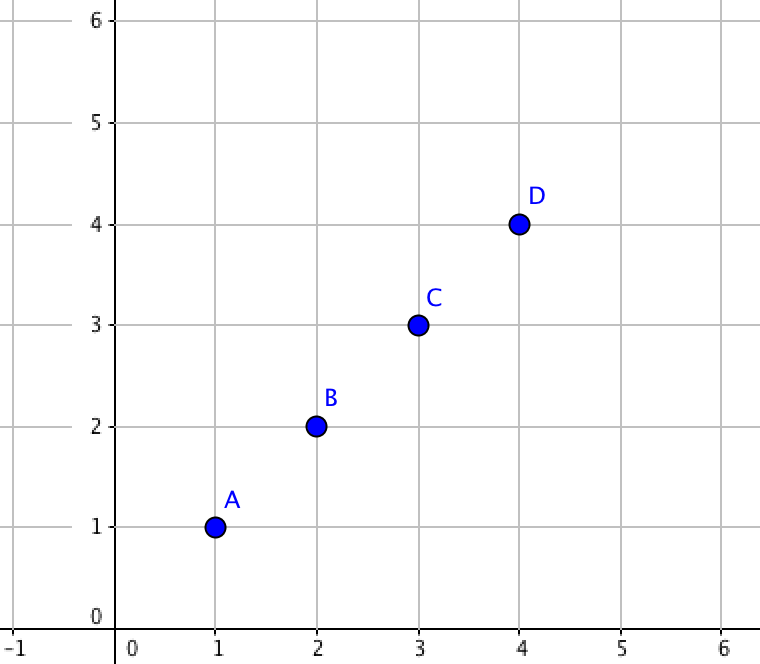
\includegraphics[width=.5\linewidth]{points.png} 
    \caption{Plotting points for the line $y=x$.} 
    \vspace{4ex}
  \end{minipage}%%
  \begin{minipage}[b]{0.5\linewidth}
    \centering
    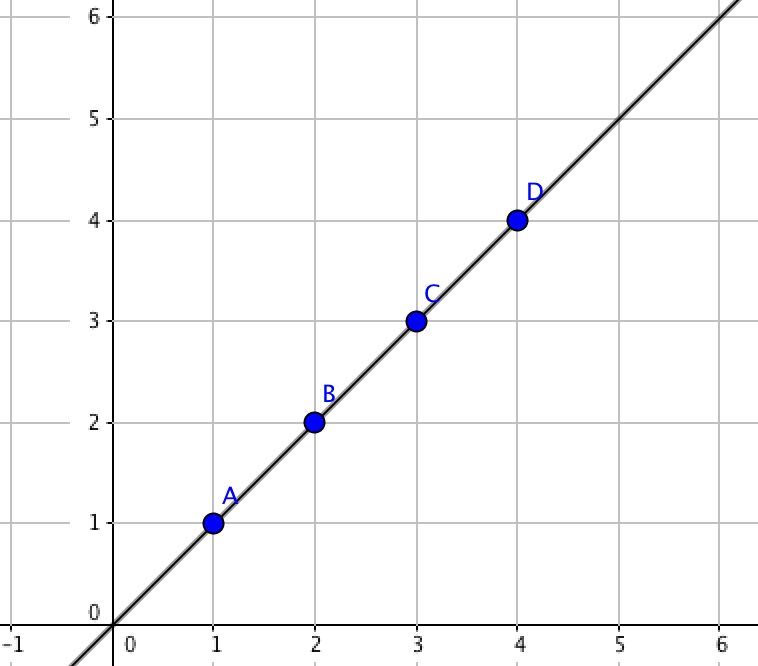
\includegraphics[width=.5\linewidth]{pointsline.png} 
    \caption{The line $y=x$.} 
    \vspace{4ex}
  \end{minipage} 
  \begin{minipage}[b]{0.5\linewidth}
    \centering
    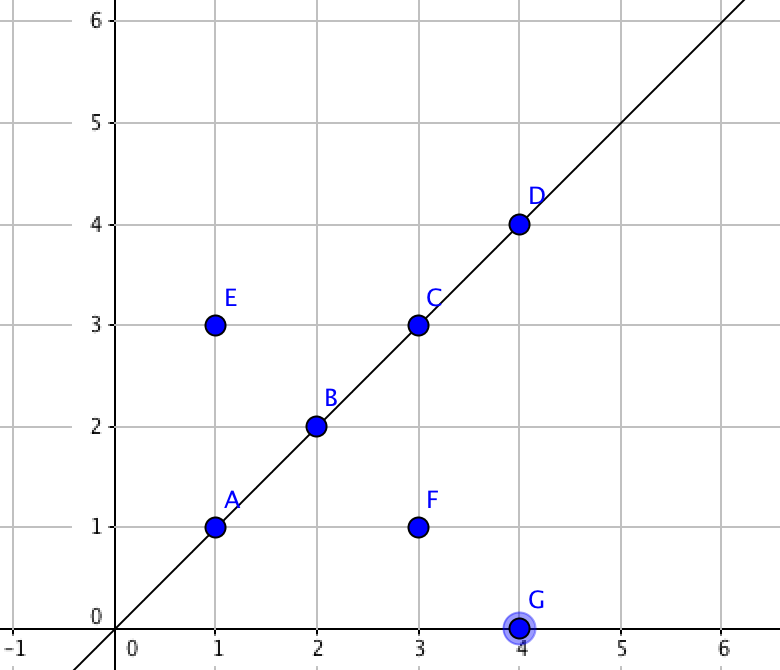
\includegraphics[width=.5\linewidth]{points2.png} 
    \caption{Plotting points for a new line.} 
    \vspace{4ex}
  \end{minipage}%% 
  \begin{minipage}[b]{0.5\linewidth}
    \centering
    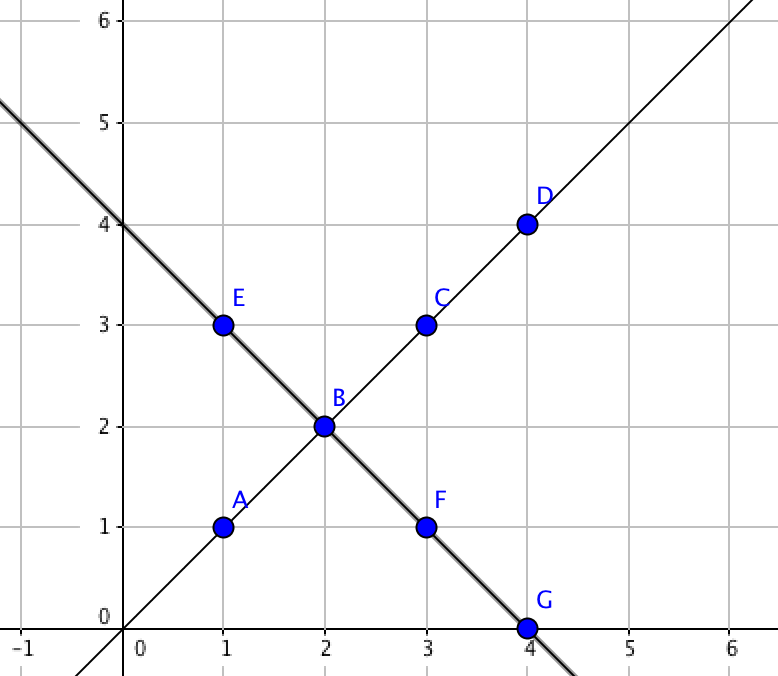
\includegraphics[width=.5\linewidth]{line2.png} 
    \caption{The lines $y=x$ and $y=-x+4$.} 
    \vspace{4ex}
  \end{minipage} 
\end{figure}


It's no coincidence that we call the objects in two sets the ``intersection''.  A single solution in the solution set of an equation is a point on the line that corresponds to that equation.  If we have two lines on a graph, the point where they intersect is a point that's on both of the lines at the same time.  That means that the point is going to be in the solution set of both equations.

\begin{example}
Find the intersection for the following system of linear equations.
$$y - 4x = -4$$
$$2y + x = 10$$

Using this strategy, we want to plot both equations.  To do this, we want them in a form that we can use to plot them, so we'll put them in slope-intercept form.
For the first line:
$$
\begin{array}{rcl}
y - 4x & = & -4 \\
y & = & 4x - 4 \end{array}$$

And for the second line:
$$\begin{array}{rcl}
2y + x & = & 10 \\
2y & = & 10 - x \\ 
y & = & 5 - \frac{x}{2} \\
y & = & - \frac{1}{2} x + 5 \end{array}$$

Plotting both lines then shows that they have an intersection.
%Insert graph
\begin{center}
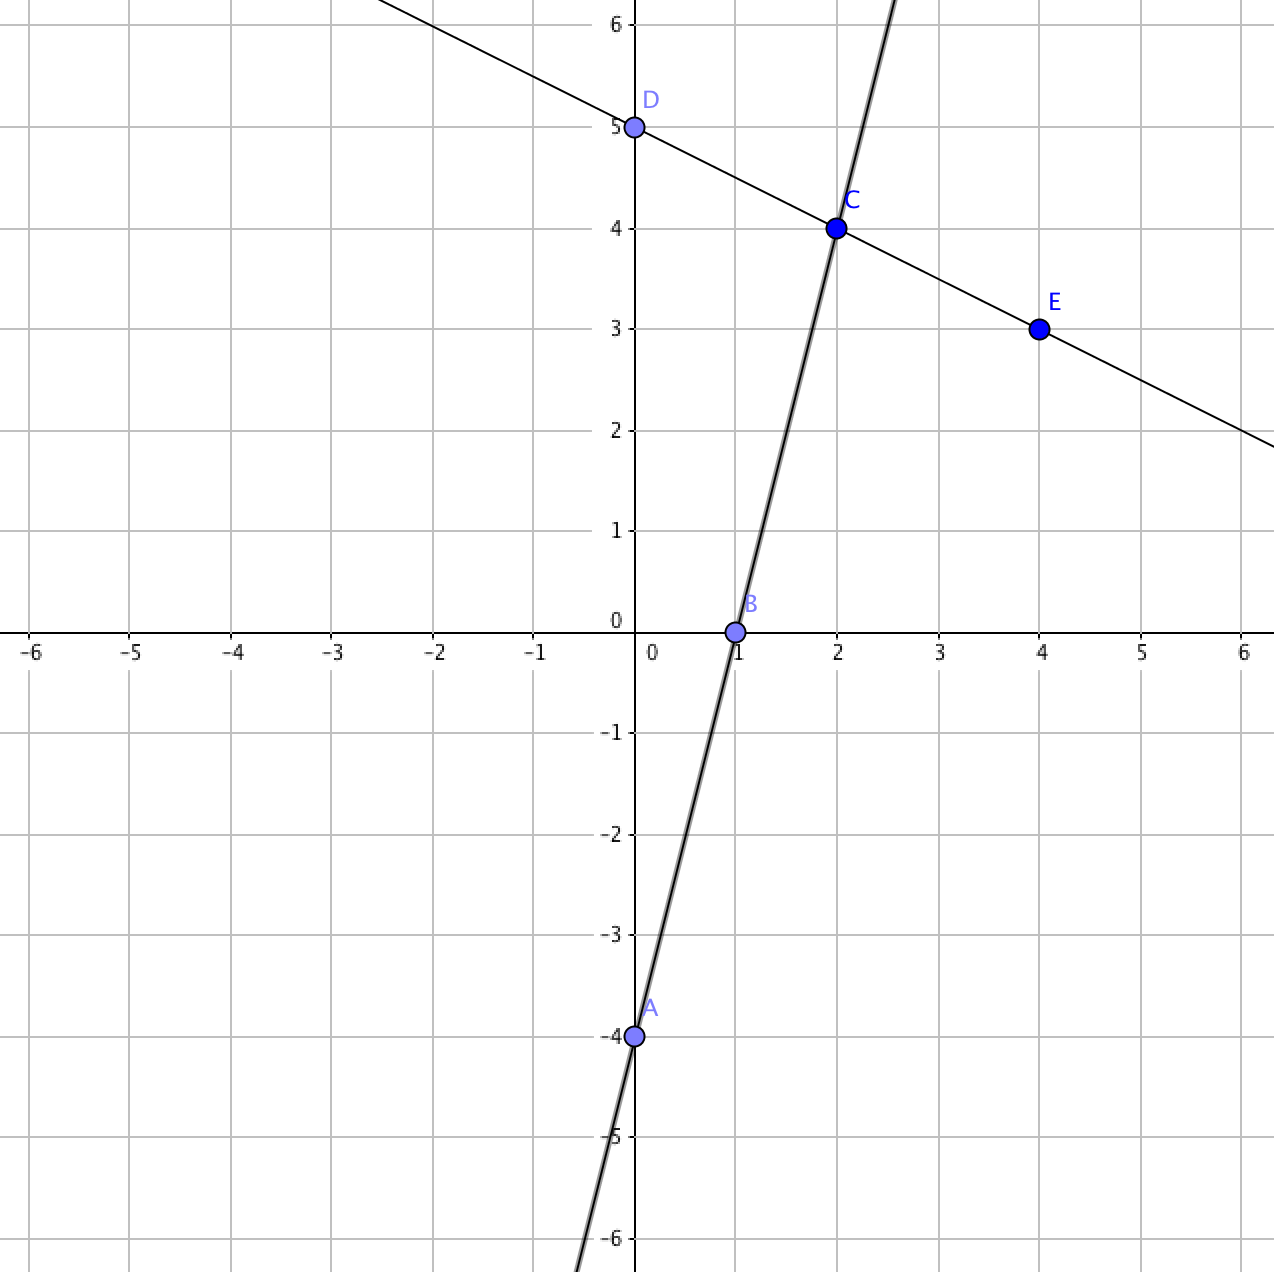
\includegraphics[scale=.35]{intersection.png}	
\end{center}

We can then see that the lines intersect at the point $(2,4)$.  This means that $(2,4)$ is in the solution set to both equations, and is thereby the solution to this system of equations.
\end{example}

This is a useful tool for finding solutions to systems of linear equations as long as being close is good enough.  Unfortunately, some systems of linear equations have solutions that aren't on the grid-lines for a particular scale.

\begin{prblm}
Consider the following system of linear equations.
$$y = -\frac{1}{2}x + 3$$
$$y = 2x$$

What do you think the intersection is?  What could you do to convince someone who didn't agree?

\vspace{4cm}
\end{prblm}


\section{Substitution}

Although most people aren't accustomed to the idea, there is more than one way to do most things in math.  This is a good thing!  If the only way to find the solution to a system of equations was to graph them and point at it, it would be pretty difficult to solve a lot of these systems.  This is where substitution comes in.  Consider two equations in slope-intercept form.

$$y = 2x + 4$$
$$y = 3x + 2$$



Well, if the right side of the first equation is equal to $y$, and the right side of the second equation is equal to $y$, they must be equal to each other!  This is the driving force of substitution.  If two things have the same value, they're equal to each other.

$$2x + 4 = 3x + 2$$

And this is single linear equation that we can solve.

$$\begin{array}{rcl}
2x + 4 & = & 3x + 2\\
4 & = & x + 2 \\
2 & = & x \end{array}$$

So now we know the solution has an $x$-value of $2$.  Nice.  So what about that $y$-value?  We can plug the $x$-value we just found into one of those equations and find out.  We'll choose the first equation.

$$\begin{array}{rcl}
y & = & 2\times2 + 4\\
y & = & 4 + 4\\
y & = & 8 \end{array}$$

Awesome.  Now we think the solution has an $x$-value of $2$, and a $y$-value of $8$.  If this is true, then $(2,8)$ must be a solution to the second equation as well.  We can check that.

$$\begin{array}{rcl}
y & = & 3x + 2 \\
8 & = & 3\times 2 + 2\\
8 & = & 6 + 2 \end{array}$$

Everything checks out.  We've found a solution to this linear system.

\pagebreak

For this last problem, the solution had nice, clean integer values for the solution.  The equations were also given in slope-intercept form.  This won't always be the case.

\begin{example}
Solve the system of linear equations.

$$\begin{array}{rcl}
4y - 16x & = & 25 \\
2y + x & = & -1 \end{array}$$

To use the substitution strategy the way we did last time, we want to solve each equation for either $y$ or $x$.  We had the equations solved for $y$ last time, and solving for $y$ should be natural to us by now, so we'll do that for now.

For the first equation:

$$\begin{array}{rcl}
4y - 16x & = & 25 \\
4y & = & 16x + 25 \\
y & = & 4x + \frac{25}{4} \end{array}$$

And for the second equation:

$$\begin{array}{rcl}
2y + x & = & -1 \\
2y & = & -x -1 \\
y & = & -\frac{1}{2}x - \frac{1}{2} \end{array}$$

Now we're in a similar position as we were at the beginning of the last problem.  We realize that both $-\frac{1}{2}x - \frac{1}{2}$ and $4x + \frac{25}{4}$ are equal to $y$, and so we set them equal to each other.

$$\begin{array}{rcl}
-\frac{1}{2}x - \frac{1}{2} & = & 4x + \frac{25}{4}\\ \\
-\frac{1}{2} & = & 4\frac{1}{2}x + \frac{25}{4}\\ \\
-\frac{1}{2} - \frac{25}{4} & = & 4\frac{1}{2}x\\ \\
-\frac{2}{4} - \frac{25}{4} & = & \frac{9}{2}x\\ \\
-\frac{27}{4} & = & \frac{9}{2}x\\ \\
-\frac{27}{4} \div \frac{9}{2}& = & x \\ \\
-\frac{3}{2} & = & x\\
\end{array}$$

So we've figured out that the solution has an $x$-value of $-\frac{3}{2}$.  Now we need to figure out the $y$-value.  Again, we plug our $x$-value into one of the equations, and the $y$-value should come out.  The great part is that, for the whole sequence where we solved for $y$ in the first equation, each of those equations is equivalent.  We can choose the new version of the first equation to find our $y$-value.

$$\begin{array}{rcl}
y & = & 4\times \left(-\frac{3}{2}\right) + \frac{25}{4}\\
y & = & -\frac{12}{2} + \frac{25}{4}\\
y & = & -\frac{24}{4} + \frac{25}{4}\\
y & = & \frac{1}{4}\\
\end{array}$$

This tells us that the point in the first equation where the $x$-value is $-\frac{3}{2}$ has a $y$-value of $\frac{1}{4}$.  Then, the solution is the point, $\left(-\frac{3}{2}, \frac{1}{4}\right)$.
\end{example}

Let's try a tougher one.

\begin{example}
Solve the system of linear equations.
$$2y - 3x = 9$$
$$5y + 2x = -10$$

For the first equation:

$$\begin{array}{rcl}
2y - 3x & = & 9\\
2y & = & 3x + 9\\
y & = & \frac{3}{2}x + \frac{9}{2} \end{array}$$

And for the second equation:

$$\begin{array}{rcl}
5y + 2x & = & -10\\
5y & = & -10 - 2x\\
y & = & -\frac{2}{5}x - 2 \end{array}$$

Now, setting the right side of each equation equal, 

$$\begin{array}{rcl}
\frac{3}{2}x + \frac{9}{2} & = & -\frac{2}{5}x - 2\\ \\
\frac{3}{2}x + \frac{2}{5}x + \frac{9}{2} & = & - 2\\ \\
\frac{3}{2}x + \frac{2}{5}x & = & -\frac{9}{2} - 2\\ \\
\frac{15}{10}x + \frac{4}{10}x & = & -\frac{9}{2} - \frac{4}{2}\\ \\
\frac{19}{10}x & = & -\frac{13}{2}\\ \\
x & = & -\frac{13}{2} \div \frac{19}{10}\\ \\
x & = & -\frac{65}{19} \\
\end{array}$$
\end{example}


\section{Elimination}

There's yet another strategy for solving systems of linear equations.  This strategy is based on a similar idea as the one the substitution strategy is based on.  Both sides of an equation are equal, and can be replaced with the other.  Consider the following linear system.

$$\begin{array}{rcl}
y - x & = & 4 \\
y + x & = & 2\end{array}$$

From the second unit, we learned that, as long as we add the same thing to both sides, the equation will still be equivalent.  For this strategy, we want to take advantage of the fact that each side of the first equation has the same value.  If we think of the equations as balanced scales, we can think of our next step as taking everything off of the second scale and putting it on the appropriate sides of the first scale.

$$\begin{array}{rcl}
y - x & = & 4 \\
y - x + (y + x) & = & 4 + (2)
\end{array}$$

The stuff in parentheses comes from the second equation.  At this point, we just want to simplify and see what happens.

$$\begin{array}{rcl}
y - x + (y + x) & = & 4 + (2)\\
y - x + y + x & = & 6\\
2y + 0x & = & 6\\
2y = 6
y = 3 \end{array}$$

What happened?

When we took everything from the second equation and put it on the first, we ended up with an equation that has a solution where both of our previous equations had solutions.  Since this value only has a $y$-value and no $x$-value, we have the beginning of a solution!  Let's put that $y$-value in and see what $x$ is.

$$
\begin{array}{rcl}
y - x & = & 4 \\
3 - x & = & 4 \\
3 & = & 4 + x \\
-1 & = & x \end{array}$$

With a value $y$ and $x$, we have a complete solution.  We call this the Elimination Method because the hope is that, when we add the equations together, one of the variables will cancel or be eliminated, leaving us with a linear equation with only one variable.  This worked out for us this time because one equation had a positive $x$, and the other equation had a negative $x$.  If we have more $x$'s in one equation than the other, we'll have some positive or negative $x$'s left over.  In order to make them cancel, we sometimes have to find an equivalent equation.

\begin{example}
Solve the following linear system using the elimination method.

$$\begin{array}{rcl}
y + 2x & = & -2\\
-2y - x & = & 3 \end{array}$$

If we take the second equation and add it to the first equation now, we'll still have an equation with two variables.

$$\begin{array}{rcl}
y + 2x + (-2y - x) & = & -2 + (3)\\
y + 2x - 2y - x & = & 1\\
-y + x & = & 1 \end{array}$$

Like before, we ended up with an equation that has a solution where both of our previous equations had solutions. Unfortunately, it still has two variables, so we can't make any conclusions about it yet.  Let's take a look at the first two equations again.  Notice that the second equation has only one negative $x$, while the first equation has two.  We want to take advantage of equivalent equations.  If we want an equation equivalent to the second equation, but which has two negative $x$'s, we can multiply both sides by 2. Then, the system

$$\begin{array}{rcl}
y + 2x & = & -2\\
-2y - x & = & 3 \end{array}$$

becomes

$$\begin{array}{rcl}
y + 2x & = & -2\\
-4y - 2x & = & 6 \end{array}$$

Because the equations we have are equivalent to the previous equations, the linear system is also equivalent; it will have all of the same solutions.  Let's try adding the equations again.

$$\begin{array}{rcl}
y + 2x + (-4y - 2x) & = & -2 + (6) \\
y + 2x -4y -2x & = & 4 \\
-3y & = & 4 \\
y & = & -\frac{4}{3}
\end{array}$$

Perfect.  We eliminated one of the variables according to plan.  We know that our solution has a $y$-value of $-\frac{4}{3}$.  We can work on finding $x$ now.  This will be easier if we start with the second equation, so we don't have to divide at the end.

$$\begin{array}{rcl}
-2y - x & = & 3 \\
-2\times \left(-\frac{4}{3}\right) - x & = & 3 \\
\frac{8}{3} - x & = & 3 \\
\frac{8}{3} & = & 3 + x \\
\frac{8}{3} - 3 & = & x \\
\frac{8}{3} - \frac{9}{3} & = & x \\
-\frac{1}{3} & = & x \end{array}$$

With values for $x$ and $y$, we can now say that we have a solution.
\end{example}

We're going to do one more example, but there's going to be a twist to it.

\begin{example}
Solve the system of linear equations.

$$\begin{array}{c}
y = \frac{3}{5}x - 6\\
3y + 2x = 1 \end{array}$$

The first thin we have to watch out for is the equals sign.  Remember that the strategy only works because we're taking everything off of one scale and putting it on the appropriate sides of the other scale.  We can't add straight down because the equals signs don't line up.  We have to make sure they do.

$$\begin{array}{rcl}
y & = & \frac{3}{5}x - 6\\
3y + 2x & = & 1 \end{array}$$

That's better.  Now we can clearly see that we need to move the $\frac{3}{5}x$ term to the other side of the first equation.

$$\begin{array}{rcl}
y - \frac{3}{5}x & = & -6\\
3y + 2x & = & 1 \end{array}$$

Now we're in a weird spot.  It looks like we would have to multiply one of the equations by a fraction in order to get the $x$'s to cancel.  Finding that fraction can sometimes take valuable time.  What we're going to do is take advantage of equivalent equations again, and we're going to fix both of the equations.  We'll look at the coefficient of the $x$ in the first equation, and multiply the second equation by it.  Then we'll look at the coefficient of $x$ in the second equation and multiple by first equation by it.  This way, the $x$'s in both equations will be multiplied by both coefficients, and this should make them cancel.


$$\begin{array}{rcl}
y - \frac{3}{5}x & = & -6\\
3y + 2x & = & 1\\ \\
y - \frac{3}{5}x & = & -6\\
\frac{3}{5}\times 3y + \frac{3}{5}\times 2x & = & \frac{3}{5}\times 1\\ \\
y - \frac{3}{5}x & = & -6\\
\frac{9}{5}y + \frac{6}{5}x & = & \frac{3}{5}\\ \\
2y - 2\times \frac{3}{5}x & = & 2\times (-6)\\
\frac{9}{5}y + \frac{6}{5}x & = & \frac{3}{5}\\ \\
2y - \frac{6}{5}x & = & -12 \\
\frac{9}{5}y + \frac{6}{5}x & = & \frac{3}{5} \end{array}$$

And now, when we add the equations together, the $x$'s will cancel.

$$\begin{array}{rcl}
2y - \frac{6}{5}x + (\frac{9}{5}y + \frac{6}{5}x) & = & -12 + (\frac{3}{5}) \\
2y - \frac{6}{5}x + \frac{9}{5}y + \frac{6}{5}x & = & -\frac{60}{5} + \frac{3}{5} \\
2y + \frac{9}{5}y & = & -\frac{57}{5} \\
\frac{10}{5}y + \frac{9}{5}y & = & -\frac{57}{5} \\
\frac{19}{5}y & = & -\frac{57}{5} \\
y & = & -\frac{57}{5} \div \frac{19}{5}\\
y & = & -3
\end{array}$$

We have a $y$-value.  What's missing?

$$\begin{array}{rcl}
3y + 2x & = & 1\\
3 \times -3 + 2x & = & 1 \\
2x & = & 10 \\
x & = & 5 \end{array}$$

This tells us that our solution is $(5,-3)$.
\end{example}

As we can see, some problems are more well-suited for elimination than others.

\pagebreak

\section*{Exercises}

\begin{exercise}
Find the slope of the line that goes through (0,6) and (2,0)
\end{exercise}

\bigskip

\begin{exercise}
Find the slope of the line that goes through (0,2) and (6,0)
\end{exercise}

\bigskip

\begin{exercise}
	Find the solution for the following linear system:
	$$
	\begin{array}{rcl}
	x & = & 4 \\
	y & = & 2x+1	
	\end{array}
	$$
	Is there one method for solving this system that is easier than the others? Give evidence for your answer. 
\end{exercise}
\bigskip

\begin{exercise}
	Find a linear system that has the solution $(2,5)$.
\end{exercise}
\bigskip

\begin{exercise}
Your philosophy teacher wants you to compare apples and oranges for an assignment. Your friend picks up a total of 12 bundles of fruit and paid \$74.00. The apples weighed 5 lbs per bundle and the oranges weighed 4 lbs per bundle. If the bundles of apples cost \$5 a piece and the bundles of oranges cost \$7 a piece, how many bundles of apples did your friend buy?
\end{exercise}
\bigskip

\begin{exercise}
Consider the linear system:
$$
\begin{array}{rcc}
y& = & x \\
y & = & -x 	
\end{array}
$$
with respective slopes 1 and -1. If we change the slopes of the two lines to 2 and -2, without changing the y-intercept, does it change the solution? If so, what is the new solution. Provide evidence for your claim. 	
\end{exercise}

\bigskip

\begin{exercise}
Solve the following system of equations using whatever method you choose:
$$
2x-y = 3
$$
$$
-3y = 4 +x
$$	
\end{exercise}

\bigskip

\begin{exercise}
	In what type of situations is it more difficult to use graphing than substitution or elimination to solve a linear system? Give an example of a system in which this is true. 
\end{exercise}

\bigskip

\begin{exercise}
Find the solution for the system:
$$
\begin{array}{rcl}
7x + 4y & = & 3 \\
x + \frac{1}{7}y & = & 3	
\end{array}
$$
\end{exercise}
\bigskip

\begin{exercise}
Solve the following system in two ways (using substitution and elimination) and compare your answers:
$$
\frac{1}{2}x + y = 6
$$	
$$
4x =y
$$

Should the solutions be the same or different. Provide evidence for your answer.
\end{exercise}

\bigskip

\begin{exercise}
It costs \$5.00 for a student and \$10.00 for non-students to see a movie at the Cinema 12. If the theater had 75 people go to a movie one night and made \$500 dollars from ticket sales, how many students saw a movie that night?
\end{exercise}

\bigskip

\begin{exercise}
	Find the solution for the linear system:
	$$
	2x+y=17
	$$
	$$
	\frac{1}{2}y=-x +1
	$$	
\end{exercise}

\bigskip

\begin{exercise}
Use whatever method you choose to find the solution for the system:
$$
\begin{array}{rcl}	
1002x + 404y &=  & 2016 \\ \\
4x + 6y &= &36
\end{array}
$$ 
\end{exercise}
\bigskip

\begin{exercise}
Solve the following linear system:
$$
2x+ y = 7 
$$
$$
\frac{1}{3}y = -\frac{2}{3}x + \frac{7}{3}
$$	
\end{exercise}

\bigskip

\begin{exercise}
Find a point on the line, and write it in point-slope form using the chosen point.
\end{exercise}

\bigskip

\begin{exercise}
Find the slope-intercept form of a line passing through the points (-1,-1) and (7,3).
\end{exercise}

\bigskip

\begin{exercise}
Choose three different slopes, and find the y-intercepts of  the lines with those slopes passing through the point (2,2).  Graph these lines on the same graph.
\end{exercise}

\bigskip

\begin{exercise}
	Consider the function $16y + 10 + x = 2x + 42$. Is this function linear? How can we tell?
\end{exercise}
